\section{Program Analysis and Abstract Interpretation}
\label{bg:sec:abstract_interpretation}

As our way of living is becoming increasingly dependent on programs, errors
in safety-critical system can incur huge expenses, and even costs of lives.
For example, the maiden flight of Ariane 5 resulted in a failure, because of
a software instruction failed to convert a 64-bit floating-point number into
16-bit signed integer, as the result is too large to be represented by a 16-bit
signed integer~\cite{dowson97}.  The Patriot defense system failed to intercept
an incoming missile because of an accumulated round-off error in the system's
internal clock, resulted in the deaths of 28 people in 1991~\cite{patriot}.
\emph{Static analysis}, a process of analyzing a piece of program written in
an \gls{hll} without executing it, is therefore a research topic of great
importance to prevent similar catastrophic errors and mitigate costs of failure
in the future.

It is unfortunate that because of the halting problem~\cite{turing37} and
a direct consequence of it, Rice's theorem~\cite{rice53}, any nontrivial
property on the outcome of a program is in general undecidable.  It means that
an interesting property, a \emph{yes} or \emph{no} question which is never
always true or always false for all programs, is \emph{undecidable}; or in
other words, it cannot be answered.  Even a question as seemingly innocuous
as \emph{``does this program return zero''} is difficult to answer.  A static
analyzer, when faced with such a question, therefore do not attempt to
produce a definite \emph{yes} or \emph{no}, instead it answers with either
a definite \emph{yes} or \emph{I don't know}~\cite{mine04}; and producing a
meaningful \emph{yes} in an efficient manner poses a challenging task to static
analyzers.  Additionally, they often rely heavily on formal techniques to
perform well.  Typical techniques employed include symbolic execution, model
checking~\cite{kroening03}, satisfiability modulo theories~\cite{demoura08},
data-flow analysis based on lattices~\cite{nielson99}, and abstract
interpretation~\cite{cousot77}.

There are static analyzers specifically tailored to prove the absence of
run-time errors in computing systems.  Astr\'ee~\cite{astree}, based on
the theory of abstract interpretation, has been successful in proving the
safety of the flight control systems of the Airbus A340 and A380 series,
and the automatic docking software of the Jules Vernes Automated Transfer
Vehicle~\cite{dasia09}.  Other static analysis tools which employ abstract
interpretation include MathWorks's Polyspace Bug Finder~\cite{polyspace},
Fluctuat~\cite{Fluctuat}, and ECLAIR~\cite{eclair}.

This section starts by introducing the data-flow analysis framework to analyze
a simple program, abstract interpretation is then applied to this example, and
the properties of the resulting analysis are further discussed.

% This is then extended to define a scalable analysis capturing accuracy.
% Later in Chapter~\ref{chp:progopt} we accommodate sequential statements,
% \iflit~branches and \whilelit~loops in the accuracy analysis, and in
% Chapter~\ref{chp:latopt}, we further improve our analysis by supporting
% multi-dimensional arrays.

\subsection{Data-Flow Analysis Framework}
\label{bg:sub:data_flow}

In this section, we use the \gls{dfa} framework~\cite{nielson99} to deduce
the semantics of a program named \verb|simple| in Figure~\ref{bg:lst:simple},
which consists of only one variable \verb|x|.  We assume an initial
set $\iota \subseteq \realset$ of values of \verb|x|, and the property
pertaining to us is whether a particular value $x_\mathrm{invalid}$ is
unreachable.  By computing the set of all reachable final values of \verb|x|,
$X$, checking $x_\mathrm{invalid} \notin X$ is sufficient.  A sensible
definition for the set of values can be reached by \verb|x| is a subset of
all real numbers $\realset$, \ie~an element of $\powersetof\realset$, where
$\powersetof\realset$ denotes the \emph{power set} of $\realset$, also known as
the set of all subsets of $\realset$.
\begin{figure}[ht]
    \centering
    \begin{minipage}{0.5\textwidth}
    \begin{lstlisting}
    float simple(float x)
    {
        while (x > 1.0)
            x *= 0.9;
        return x;
    }
    \end{lstlisting}
    \end{minipage}
    \caption{%
        A simple program example to be statically analyzed.
    }\label{bg:lst:simple}
\end{figure}

The first step of \gls{dfa} is to translate the body of \verb|simple| into a
\gls{cdfg}, as shown in Figure~\ref{bg:fig:cdfg} where each block consists of
a single statement or conditional, and the edges in the graph model the data-
and control-flows.  The \textbf{tt} and \textbf{ff} respectively highlight
the control-flow branch taken when the conditional \mbox{``\texttt{x < 1}''}
evaluates to either true or false.
\begin{figure}[ht]
    \centering
    \tikzstyle{block} = [
        draw,
        fill=white,
        rectangle,
        minimum height=2em,
        minimum width=4em
    ]
    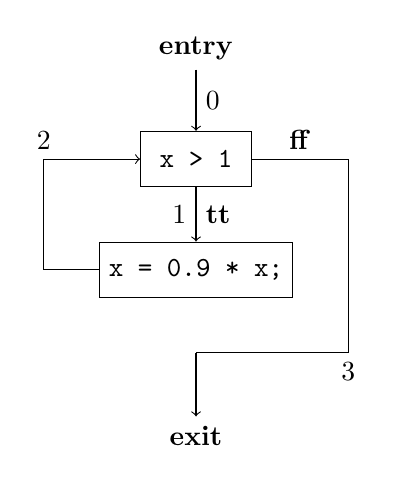
\begin{tikzpicture}[node distance=4em]
        \node(entr) {\textbf{entry}};
        \node(cond) [block, below of=entr] {\texttt{x > 1}};
        \node(stmt) [block, below of=cond] {\texttt{x = 0.9 * x;}};
        \node(midl) [coordinate, left of=stmt, xshift=-1.5em] {};
        \node(midr) [coordinate, right of=stmt, xshift=1.5em] {};
        \node(rtrn) [coordinate, below of=stmt, yshift=1em]
            {\texttt{return x;}};
        \node(exit) [below of=rtrn, yshift=1em] {\textbf{exit}};
        \draw[->] (entr) -- node[auto]{0} (cond);
        \draw[->] (cond) -- node[right]{\textbf{tt}} node[left]{1} (stmt);
        \draw[- ] (stmt) -- (midl);
        \draw[->] (midl) |- node[auto]{2} (cond);
        % \draw[->] (stmt) to[out=180, in=180] (cond);
        \draw[- ] (cond) -| node[auto, near start]{\textbf{ff}} (midr);
        \draw[- ] (midr) |- node[auto]{3} (rtrn);
        % \draw[->] (cond) to[out=0, in=0] (rtrn);
        \draw[->] (rtrn) -- (exit);
    \end{tikzpicture}
    \caption{%
        The \gls{cdfg} of \texttt{simple} in Figure~\ref{bg:lst:simple}.
    }\label{bg:fig:cdfg}
\end{figure}

The individual blocks in the \gls{cdfg} can therefore be defined as functions
$f: \powersetof\realset \to \powersetof\realset$ that admits an $S$ and
produces $T$, where both $S$ and $T$ are elements of $\powersetof\realset$.
For instance, for the statement ``\texttt{x *= 0.9;}'' a function $f_1$ can be
defined as follows:
\begin{equation}
    f_1(S) = \{ 0.9 v \mid v \in S \}.
\end{equation}
Here, the definition of $f_1$ indicates that for all possible input values
$v$ of \verb|x| in the set $S$, we multiply it by $0.9$ and collect the
multiplied results into a new set as the output of $f_1$.  Similarly, because
\mbox{``\texttt{x > 1}''} has two conditional branches, two functions,
$f_{2,\truelit}$ and $f_{2, \falselit}$, respectively for both true- and
false-branches of it can be defined:
\begin{equation}
    \begin{aligned}
        f_{2, \truelit}(S) &= S \cap \{ v \in \realset \mid v > 1 \}, \\
        f_{2, \falselit}(S) &= S \cap \{ v \in \realset \mid v \leq 1 \}.
    \end{aligned}
\end{equation}
where $X \cap Y$ computes the intersection of the two sets $X$ and $Y$.

In the next step, the edges of the \gls{cdfg} are labelled with numbers 0, 1,
2 and 3 to signify different locations of the program.  For each edge labelled
$i$, it is now possible to compute an $A(i)$, a set of values that could be
reached by \verb|x| in a program execution at each location $i$, by wiring up
the functions $f_1$, $f_{2, \truelit}$ and $f_{2, \falselit}$ that correspond
to program statements.  This gives rise to the following system of data-flow
equations:
\begin{align}
    A(0) &= \iota,
        \label{bg:eq:dfa0} \\
    A(1) &= f_{2, \truelit}(A(0) \cup A(2)),
        \label{bg:eq:dfa1} \\
    A(2) &= f_1(A(1)),
        \label{bg:eq:dfa2} \\
    A(3) &= f_{2, \falselit}(A(0) \cup A(2)),
        \label{bg:eq:dfa3}
\end{align}
where $A(0) \cup A(1)$ is the union of $A(0)$ and $A(1)$.

Unfortunately, computationally solving this system of equations is not an
easy task.  In the rest of this section, the two significant impediments
are explained, and subsequently, theories are introduced to unravel them.
Section~\ref{bg:sub:lfp} discusses how the system of \gls{dfa} equations can
be solved analytically for the most desired solution, using a minimal set of
reachable values for $A(1)$ as an example.  However, this analytical solution
cannot be computed by a machine.  By building on top of this foundation,
Section~\ref{bg:sub:intervals} therefore provides a practical solution to
compute a safe approximation of this set by an algorithm.


\subsection{Least Fixpoint Solution to a Data-Flow Analysis Problem}
\label{bg:sub:lfp}

There are multiple solutions to this system.  For example, we can solve
it manually by substituting $A(0)$ and $A(2)$ in~\eqref{bg:eq:dfa1}
with~\eqref{bg:eq:dfa0} and~\eqref{bg:eq:dfa2}.  We arrive at:
\begin{equation}
    A(1) = \left(
        \iota \cup \left\{ 0.9 v \mid v \in A(1) \right\}
    \right) \cap \{ v \in \realset \mid v > 1 \}.
    \label{bg:eq:dfa_a1}
\end{equation}
It turns out that the set of all real numbers greater than $1$, or:
\begin{equation}
    A(1) = \{ v \in \realset \mid v > 1 \}
    \label{bg:eq:a11}
\end{equation}
is a solution to~\eqref{bg:eq:dfa_a1}.  Substituting $A(1)$ in the right-hand
side of~\eqref{bg:eq:dfa_a1} with this value proves that it is indeed the
solution for this equation, assuming all sets below are subsets of $\realset$
to simplify the derivation:
\begin{equation}
    \begin{aligned}
        A(1)
        &= \bigg( \iota \cup \Big\{ 0.9 v \mid v \in
                \left\{ v^\prime \mid v^\prime > 1 \right\}
           \Big\} \bigg) \cap \{ v \mid v > 1 \} \\
        &= \bigg( \iota \cup \left\{ 0.9 v \mid v > 1 \right\} \bigg) \cap
           \{ v \mid v > 1 \}
         = \bigg( \iota \cup \left\{ v \mid v > 0.9 \right\} \bigg) \cap
           \{ v \mid v > 1 \} \\
        &= \bigg( \iota \cap \{ v \mid v > 1 \} \bigg) \cup
           \bigg(
               \left\{ v \mid v > 0.9 \right\} \cap \{ v  \mid v > 1 \}
           \bigg) \\
        &= \bigg( \iota \cap \{ v \mid v > 1 \} \bigg) \cup
           \{ v \mid v > 1 \}
         = \{ v \mid v > 1 \}.
    \end{aligned}
\end{equation}

Intuitively, a manual inspection of \verb|simple| finds that \verb|x| can
reach values $v$, $0.9 v$, $0.9^2 v$, and so on, such that all values in this
sequence are greater than $1$, for each $v \in \iota$; or more succinctly, an
alternative solution to $A(1)$ should be:
\begin{equation}
    A(1) = \{ v \in \iota \mid 0.9^k v > 1 \wedge k \in \naturalset \},
    \label{bg:eq:a12}
\end{equation}
where $k \in \naturalset$ denotes $k$ is one of $0, 1, 2, \mathellipsis$, \ie~a
natural number.

It is evident to us the latter solution~\eqref{bg:eq:a12} is more precise,
hence more desirable, than the former~\eqref{bg:eq:a11}.  Not only does it
contain information the former has, \ie~all values reachable by $A(1)$ is
greater than 1, it also expresses the fact that it only consists of values of
the form $0.9^k v$, where $v \in \realset$ and $k \in \naturalset$.  A useful
definition of preciseness is therefore the subset relation ``$\subseteq$''.
If it is known that $X \subseteq X^\prime$, and $X$ and $X^\prime$ are both
solution to a system of data-flow equations, then $X$ is clearly more appealing
than $X^\prime$.

The set $\powersetof\realset$, with a preciseness ordering ``$\subseteq$'',
is a \emph{partially ordered set}.  It has three following properties for any
$X, Y, Z \in \powersetof\realset$: it is \emph{reflexive}, $X \subseteq X$; it
has the \emph{antisymmetry} property, \ie~if $X \subseteq Y$ and $Y \subseteq
X$, then $X = Y$; and finally it is transitive, if $X \subseteq Y$ and $Y
\subseteq Z$, then $X \subseteq Y$.  In contrast to a total order such as the
set of reals $\realset$, not every two elements in $\powersetof\realset$ can be
compared, \eg~neither of the sets $\{1, 2, 3\}$ and $\{2, 3, 4\}$ is a subset
of one another.

For the purpose of computing the solution to $A(1)$'s
equation~\eqref{bg:eq:dfa_a1}, a function $f: \powersetof\realset \to
\powersetof\realset$ can be defined:
\begin{equation}
    f(X) = \left(
        \iota \cup \left\{ 0.9 v \mid v \in X \right\}
    \right) \cap \{ v \in \realset \mid v > 1 \},
    \label{bg:eq:a1_transfer}
\end{equation}
so that all solutions of the original equation~\eqref{bg:eq:dfa_a1} are now in
this following set, which are known as the \emph{fixpoints}\footnotemark[1] of
$f$:
\begin{equation}
    \mathrm{Fix}(f) = \left\{
        X \in \powersetof\realset \mid
        f(X) = X
    \right\}.
\end{equation}
\footnotetext[1]{%
    Another common name for \emph{fixpoint} is \emph{fixed point}.  To avoid
    being mistaken for the fixed point representation, a binary number
    representation, the term \emph{fixpoint} is used instead.
}

By using this particular definition of preciseness, two important questions
arise:
\begin{enumerate}

    \item Is the most precise solution unique?  A unique most precise solution
    is defined as the only one which is the most precise among all possible
    solutions to the systems of data-flow equations.  In other words, if
    it exists, then it is defined as the \emph{least fixpoint} (\gls{lfp}) of
    $f$ which is a subset of all other fixpoints, \ie~$\lfp (f) \subseteq
    \mathrm{Fix}(f)$.  As we have discussed earlier, multiple fixpoints exist,
    and it is possible that these fixpoint solutions are not comparable.

    \item If a unique solution exists and it is unique, how do we find it?
    This is equivalent to finding a way to compute the \gls{lfp} $\lfp(f)$
    using $f$.

\end{enumerate}

As it turns out, the first question can be answered by
Theorem~\ref{bg:thr:tarski}~\cite{tarski55, nielson99}, which proves that $\lfp
(f)$ is indeed unique.
\begin{theorem}
    \textup{[Tarski's fixpoint theorem]}
    If $\mathsf{L}$ is a complete lattice\footnotemark[2], and a function
    $g: \mathsf{L} \to \mathsf{L}$ is a monotone function, then $\lfp(g)$,
    the \gls{lfp} of $g$, is the greatest lower bound of all fixpoints
    $\mathrm{Fix}(g)$.\label{bg:thr:tarski}
\end{theorem}
\footnotetext[2]{%
    Exact definitions of \emph{complete lattice} and \emph{complete partial
    order} are not required in this section.  Both of them can be found
    in~\cite{nielson99}.
}

In our case, $f$ is a \emph{monotone} function, because by definition a
\emph{monotone} function satisfies the condition that if $X \subseteq Y$,
then $g(X) \subseteq g(Y)$.  In the \gls{dfa} of \verb|simple|, $\mathsf{L}
= \powersetof\realset$, which is a complete lattice, since all power sets
are complete lattices~\cite{nielson99}.  The \gls{lfp} of $f$, that is the
intersection of all elements in $\mathrm{Fix}(f)$, is given by this equation:
\begin{equation}
    \lfp (f) = \bigcap \mathrm{Fix}(f),
\end{equation}
which implies that $\lfp (f) \subseteq Z$ for all fixpoints $Z \in
\mathrm{Fix}(f)$, thus $\lfp (f)$ is the unique and most precise solution we
are looking for.

Secondly, another theorem~\cite{kleene52}, which is closely
related to Theorem~\ref{bg:thr:tarski}, states:
\begin{theorem}
    \textup{[Kleene's fixpoint theorem]}
    If $\mathsf{L}$ is a \gls{cpo}\footnotemark[2], and $g: \mathsf{L} \to
    \mathsf{L}$ is a Scott-continuous function, then the $\lfp (g)$ can be
    computed as the least upper bound of all values in the sequence $\bot$,
    $g(\bot)$, $g^2(\bot)$, $g^3(\bot)$, \textellipsis{}\label{bg:thr:kleene}
\end{theorem}
Here, $\bot$ denotes the least element in $\mathsf{L}$.  A function of the form
$h^n(x)$, where $h: \mathsf{M} \to \mathsf{M}$ for any domain $\mathsf{M}$ and
$n \in \naturalset$, is recursively defined as:
\begin{equation}
    h^n(x) = \left\{
        \begin{aligned}
            & h(h^{n-1}(x)) \quad && \text{if~} n > 0, \\
            & x && \text{if~} n = 0.
        \end{aligned}
    \right.
\end{equation}

Our function $f$ is \emph{Scott-continuous}: it is monotone; and for any chain
of $X_0 \subseteq X_1 \subseteq X_2 \subseteq X_3 \subseteq \mathellipsis$,
where $X_i \in \powersetof\realset$:
\begin{equation}
    \bigcup_{i \in \naturalset} f(X_i) = f \left(
        \bigcup_{i \in \naturalset} X_i
    \right).
\end{equation}
As a \gls{cpo} is more general that a complete lattice, and the least
element in $\powersetof\realset$ is the empty set $\varnothing$, using
Theorem~\ref{bg:thr:kleene} in our example analysis, the most precise solution
of $A(1)$ can therefore be computed using:
\begin{equation}
    \lfp (f) = \bigcup_{k \in \naturalset} f^k (\varnothing).
\end{equation}
The functions $f^k(\varnothing)$ for the first $k+1$ iterations can be
evaluated as follows:
\begin{equation}
    \begin{aligned}
        f^0(\varnothing) &= \varnothing, \quad\quad
        f^1(\varnothing) = \iota \cap \{ v \mid v > 1 \}, \\
        f^2(\varnothing) &= f(f^1(\varnothing))
               = \left(
                     \iota \cup
                     \{ 0.9v \mid v \in \iota \}
                 \right) \cap \{ v \mid v > 1 \}, \\
        f^3(\varnothing) &= \left(
                     \iota \cup
                     \{ 0.9v \mid v \in \iota \} \cup
                     \{ 0.9^2 v \mid v \in \iota \}
                 \right) \cap \{ v \mid v > 1 \}, \mathellipsis, \\
        f^k(\varnothing) &= \left(
                     \iota \cup
                     \{ 0.9v \mid v \in \iota \} \cup
                     \mathellipsis \cup
                     \{ 0.9^{k-1} v \mid v \in \iota \}
                 \right) \cap \{ v \mid v > 1 \}.
    \end{aligned}
\end{equation}
Finally, the most precise solution to~\eqref{bg:eq:dfa_a1} can be computed
using the \gls{lfp} formula for $f$, which is exactly the same as the
alternative solution that was manually computed in~\eqref{bg:eq:a12}:
\begin{equation}
    \begin{aligned}
        \lfp (f)
            &= \bigcup_{k \in \naturalset} f^k (\varnothing)
             = \{ v \mid v > 1 \} \cap
               \bigcup_{k \in \naturalset} \{ 0.9^k v \mid v \in \iota \} \\
            &= \{ v \in \iota \mid 0.9^k v > 1 \wedge k \in \naturalset \}.
    \end{aligned}
\end{equation}

Even though we have derive a method to statically analyze a program,
significant obstacles stymie the efficient usage of it.  Firstly, in the case
study of \verb|simple|, because the \gls{lfp} is evaluated as the union of
$f^k(\varnothing)$ in a sequence, this sequence is likely to be infinite, and
thus cannot be computed fully.  Secondly, the set of input values, $\iota$,
not only determines the number of iterations necessary in order to calculate
the \gls{lfp}, but also impacts the amount of computation required in each
iteration.  For instance if $\iota = {4}$ then it is only necessary to track
the computation for a single input value $4$, whereas when $\iota = \{ v \mid
0 \leq v \leq 1000 \}$, there are infinitely many values in the set.  As
a result, in general, the \gls{lfp} of an arbitrary self-map function $f:
\mathsf{L} \to \mathsf{L}$, where $\mathsf{L}$ is a complete lattice, is thus
not computable in finite amount of time.  In Section~\ref{bg:sub:intervals},
a method known as abstract interpretation is introduced to overcome the
computability problem.


\subsection{Abstract Interpretation with Intervals}
\label{bg:sub:intervals}

A framework of methods, known as \gls{ai}, is proposed by Cousot
\etal~\cite{cousot77} to formally mitigate the problem of computability
in program analysis.  Instead of finding the \gls{lfp}, which may not be
computable, it is much more efficient to work out an \emph{approximation} of
the \gls{lfp}\@.  Despite the outcome of an \gls{ai}-based static analysis not
as precise as the \gls{lfp}, the significant benefits of \gls{ai} is two-fold.
Firstly, the program analysis framework can now produce a ``yes'' or ``I don't
know'' answer to a query of program property in a finite amount of time.
Secondly, it provides the means to prove the correctness of an answer produced
by the static analyzer using \gls{ai} in formal mathematics.

Here a simple formulation of interval arithmetic is first introduced, which
is then exercised in the \gls{ai} framework, again by using the \verb|simple|
example in Figure~\ref{bg:lst:simple}.

\subsubsection{Interval Arithmetic}
\label{bg:ssub:interval}

\Gls{ia}, is a method to enclose a set of solutions that may arise in
computation problems~\cite{moore}.  The standard method, is to use a pair of
the form $\interval{a}{b}$, to represent $\{ v \mid a \leq v \leq b \}$, or a
set of real numbers between $a$ and $b$.  As it is closely related to sets of
reals and real arithmetic, \gls{ia} gets the benefits of both worlds.

Firstly, operations, similar to the set operations such as the subset relation
``$\subseteq$'', union ``$\cup$'' and intersection ``$\cap$'' from $\realset$,
can also be defined for real intervals $\intervalset$, and indeed real
intervals form a complete lattice.  The corresponding operations are known
as the partial ordering ``$\sqsubseteq$'', \emph{join} ``$\join$'' and
\emph{meet} ``$\meet$''.  The definitions of these operators on two intervals
$\interval{a}{b}$ and $\interval{c}{d}$ are as follows:
\begin{equation}
    \arraycolsep=0.5ex
    \begin{array}{lcll}
        \interval{a}{b} & \sqsubseteq & \interval{c}{d}
            &\defeq a \geq c \wedge b \leq d, \\
        \interval{a}{b} & \join & \interval{c}{d}
            &\defeq [\min(a, c), \max(b, d)], \\
        \interval{a}{b} & \meet & \interval{c}{d}
            &\defeq \left\{
                \begin{aligned}
                    & [\max(a, c), \min(b, d)] \quad &&
                        \text{if~} \max(a, c) \leq \min(b, d), \\
                    & \bot && \text{otherwise}.
                \end{aligned}
            \right.
    \end{array}\label{bg:eq:interval_relations}
\end{equation}
where $s \defeq t$ indicates $s$ is defined as $t$, $\min(x, y)$ and $\max(x,
y)$ respectively compute the minimum and maximum of $x$ and $y$, and $\bot$,
$\top$ respectively denote intervals with no elements, \ie~an empty interval,
and the entire set of reals.  For completeness, the above relations can be
further extended for $\top$ and $\bot$, where $X^\sharp \in \intervalset$ is an
interval:
\begin{equation}
    \begin{aligned}
        X^\sharp \join \top &\defeq \top, \\
        X^\sharp \meet \bot &\defeq \bot.
    \end{aligned}
\end{equation}
As a consequence, $\bot$ and $\top$ are respectively the least and greatest
elements of $\intervalset$.  It means that $\bot \sqsubseteq X^\sharp$ and
$X^\sharp \sqsubseteq \top$ for any interval $X^\sharp$.

Secondly, in a similar fashion to real arithmetic, arithmetic operations can
also be defined for real intervals:
\begin{equation}
    \begin{aligned}
        \interval{a}{b} + \interval{c}{d} &= \interval{a + c}{b + d}, \\
        \interval{a}{b} - \interval{c}{d} &= \interval{a - d}{b - c}, \\
        \interval{a}{b} \times \interval{c}{d}
            &= \interval{\min(s)}{\max(s)}, \\
        \text{where~} s &= \left\{
            a \times c, a \times d, b \times c, b \times d
        \right\}.
    \end{aligned}
    \label{bg:eq:interval_operations}
\end{equation}
A scalar value $x$, which can be abbreviated by $x$ itself, represents an
interval $\interval{x}{x}$ in interval arithmetic.

\subsubsection{An Informal Approach to Approximation}
\label{bg:ssub:informal}

\Gls{ai} is a theoretical framework to approximate mathematical objects
that are not directly computable.  We start by explaining what it means to
\emph{approximate}, then show how an approximation can be proved to be safe.

In the \gls{dfa} example, we arrived at a function $f: \powersetof\realset
\to \powersetof\realset$ defined by~\eqref{bg:eq:a1_transfer}, which
is not directly computable.  Interval arithmetic introduced in
Section~\ref{bg:ssub:interval} could serve as an inspiration to produce yet
another function $\tilde{f}: \intervalset \to \intervalset$, which is very
similar to the original $f$:
\begin{equation}
    \tilde{f}(X^\sharp) = \left(
        \iota^\sharp \join \left( 0.9 X^\sharp \right)
    \right) \meet [1, \infty],
    \label{bg:eq:a1_transfer_interval}
\end{equation}
where $\iota^\sharp$ is an interval that bounds the set of initial values
$\iota$.  There are two noticeable differences between $f$ and $\tilde{f}$.
Firstly, the domain, where $\tilde{f}$ carries out its computation, is
$\intervalset$ instead of $\powersetof\realset$.  Secondly, because the domain
used is different from $f$, the function definition is therefore updated
accordingly for $\tilde{f}$.

When given an input $X$, $f$ must enumerate on all $X$ to compute the result
$f(X)$ precisely.  As we have discussed earlier this is infeasible as $X$
could contain infinite number of values.  Conversely, $\tilde{f}$ does not
suffer from this problem, since~\eqref{bg:eq:interval_operations} dictates any
interval arithmetic operations can be performed by \emph{finite} number of
arithmetic computations in real.

As both Theorems~\ref{bg:thr:tarski} and~\ref{bg:thr:kleene} hold for
$\intervalset$ and $tilde{f}$, its \gls{lfp}, an approximation to the \gls{lfp}
to $f$, can therefore be computed as follows:
\begin{equation}
    \lfp (\tilde{f}) = \bigsqcup_{k \in \naturalset} \tilde{f}^k (\bot).
\end{equation}
For example, consider the case when $\iota = [0, 10]$,
\begin{equation}
    \begin{aligned}
        \tilde{f}^0 (\bot) &= \bot, \\
        \tilde{f}^1 (\bot) &= \left(
                [0, 10] \join 0.9 \bot
            \right) \meet [1, \infty] = [1, 10], \\
        \tilde{f}^2 (\bot) &= \left(
                [0, 10] \join \left( 0.9 \times [1, 10] \right)
            \right) \meet [1, \infty] = [1, 10].
    \end{aligned}
\end{equation}
As all other values in the sequence evaluates to $[1, 10]$, $\lfp(\tilde{f})$
is hence $[1, 10]$, which was computed in 3 iterations.  It is easy to see
in Figure~\ref{bg:lst:simple} that the reachable values of \verb|x| before
executing the statement ``\verb|x *= 0.9;|'' is indeed $[1, 10]$.

In many cases, an algorithm to compute $\tilde{f}^k(\bot)$ can terminate.
It is clear that if $\tilde{f}^k(\bot) = \tilde{f}^{k+1}(\bot)$ for some
$k \in \naturalset$, then for all integers $j$ that is greater than $k$,
$\tilde{f}^{j}(\bot) = \tilde{f}^{k}(\bot)$ and there is no point in computing
$\tilde{f}^{j}(\bot)$.  Widening and narrowing operators~\cite{cousot77,
nielson99} can be used to reduce the number of iterations required to reach
a fixpoint, hence accelerating, or even ensuring, termination by sacrificing
precision of the computed fixpoint, \ie~the result is no longer the \gls{lfp},
but is a fixpoint $X \sqsupseteq \lfp(\tilde{f})$ that can be computed more
easily.

\subsubsection{Gal\"ois Connection}
\label{bg:ssub:galois}

Although our informal derivation gives us an empirical evidence of the
usefulness and correctness of intervals in place of real sets, a series of
questions pertaining the theory behind it remain.  The questions are of the
format ``\emph{is $X$ a correct abstraction of $Y$}'', where $X$ and $Y$
refer to each of the following pairs: $(\intervalset, \powersetof\realset)$,
$(\tilde{f}, f)$, and $(\lfp (\tilde{f}), \lfp (f))$.

Fortunately, Cousot~\etal~\cite{cousot77} show that if a \emph{Gal\"ois
connection} can be formed between $\powersetof\realset$ and $\intervalset$,
then all of the above questions can be now answered with a resounding
``\emph{yes}''.  If $f \circ g (x)$ denotes $f(g(x))$, we can
define~\cite{nielson99}:
\begin{definition}
    \textup{[Gal\"ois connection]}
    A Gal\"ois connection is a relation between two complete lattices
    $\lattice{\mathsf{L}}{\subseteq}$ and $\lattice{\mathsf{M}}{\sqsubseteq}$,
    given by a duo of functions $\alpha: \mathsf{L} \to \mathsf{M}$ and
    $\gamma: \mathsf{M} \to \mathsf{L}$, such that for all $l \in \mathsf{L}$
    and $m \in \mathsf{M}$:
    \begin{equation}
        \alpha (l) \sqsubseteq m
        \quad
        \text{~if and only if~}
        \quad
        l \subseteq \gamma (m),
        \label{bg:eq:galois}
    \end{equation}
    alternatively the following property may sometimes be easier to work with:
    \begin{equation}
        l \subseteq \gamma(\alpha(l))
        \quad
        \text{~and~}
        \quad
        \alpha(\gamma(m)) \sqsubseteq m.
        \label{bg:eq:galois_alt}
    \end{equation}
\end{definition}\vspace{-16.5pt}
The Gal\"ois connection above can often be concisely written as:
\begin{equation}
    \lattice{\mathsf{L}}{\subseteq}
        \galois{\alpha}{\gamma}
    \lattice{\mathsf{M}}{\sqsubseteq}.
\end{equation}
Here, the functions $\alpha$ and $\gamma$ are often called the
\emph{abstraction} function and \emph{concretization} function respectively.

Bearing on the informal approach in Section~\ref{bg:ssub:informal}, the
following Gal\"ois connection can be established to formalize it:
\begin{equation}
    \lattice{\powersetof\realset}{\subseteq}
    \galois{\alpha}{\gamma}
    \lattice{\intervalset}{\sqsubseteq},
\end{equation}
The functions $\alpha: \powersetof\realset \to \intervalset$ and $\gamma:
\intervalset \to \powersetof\realset$ that satisfy~\eqref{bg:eq:galois} can be
defined as follows:
\begin{equation}
    \begin{aligned}
        \alpha(X) &= \interval{\inf(X)}{\sup(X)}, \\
        \gamma\left(
            \interval{\underline{X^\sharp}}{\overline{X^\sharp}}
        \right) &= \left\{
            v \mid \underline{X^\sharp} \leq v \leq \overline{X^\sharp}
        \right\},
    \end{aligned}
\end{equation}
where $\inf(X)$ and $\sup(X)$ are respectively the infimum and supremum of $X$.

Furthermore, from a function $g: \mathsf{L} \to \mathsf{L}$, the
\gls{ai} framework allows an approximated function $g^\sharp:
\mathsf{M} \to \mathsf{M}$ to be inductively abstracted by the Gal\"ois
connection~\cite{nielson99}.  For example, consider~\eqref{bg:eq:a1_transfer}
which is not computable, an approximated candidate $f^\sharp$ can be
computed by $\alpha \circ f \circ \gamma$.  Since we are computing in
$\intervalset$, we assume that $\iota = \gamma(\iota^\sharp)$ and $X^\sharp =
\interval{\underline{X^\sharp}}{\overline{X^\sharp}}$:
\begin{equation}
    \begin{aligned}
        f^\sharp(X^\sharp)
        &= \alpha \left( f \left(
            \gamma \left( X^\sharp \right)
        \right) \right)
        = \alpha \left( f \left( \left\{
            v \mid \underline{X^\sharp} \leq v \leq \overline{X^\sharp}
        \right\} \right) \right) \\
        &= \alpha \left(
        \left(
            \iota \cup
            \left\{
                0.9 v \mid
                \underline{X^\sharp} \leq v \leq \overline{X^\sharp}
            \right\}
        \right) \cap \{ v \mid v > 1 \} \right) \\
        &= \alpha \left(
            \left( \iota \cap \{ v \mid v > 1 \} \right) \cup
            \left( \left\{
                v \mid
                0.9 \underline{X^\sharp} \leq v \leq 0.9 \overline{X^\sharp}
            \right\} \cap \{ v \mid v > 1 \} \right)
        \right).
    \end{aligned}
\end{equation}
We introduce $\epsilon$ to denote an arbitrarily small positive value.  Because
$\alpha(A \cup B) = \alpha(A) \sqcup \alpha(B)$:
\begin{equation}
    \begin{aligned}
        f^\sharp(X^\sharp)
        ={} & \alpha \left( \left\{
            v \mid \underline{\iota^\sharp}
                \leq v \leq \overline{\iota^\sharp}
        \right\} \cap \{ v \mid v > 1 \} \right) \sqcup \\
        &
        \alpha \left( \left\{
            v \mid
            \min(0.9 \underline{X^\sharp}, 1 + \epsilon)
                \leq v \leq 0.9 \overline{X^\sharp}
        \right\} \right),
    \end{aligned}
\end{equation}
The term $\epsilon$ vanishes when the abstraction function $\alpha$ is applied:
\begin{equation}
    \begin{aligned}
        f^\sharp(X^\sharp)
        &= \alpha \left( \left\{
            v \mid
            \min(\underline{\iota^\sharp}, 1 + \epsilon)
                \leq v \leq \overline{\iota^\sharp}
        \right\} \right) \sqcup
        \left( \interval{
            \min(\underline{0.9X^\sharp}, 1)
        }{\overline{0.9X^\sharp}} \right) \\
        &= \left( \iota^\sharp \sqcap \interval{1}\infty \right) \sqcup
           \left( 0.9 X^\sharp \sqcap \interval{1}\infty \right)
         = \left( \iota^\sharp \sqcup 0.9 X^\sharp \right) \sqcap
           \interval{1}\infty.
    \end{aligned}
\end{equation}
which is identical to $\tilde{f}$ defined
in~\eqref{bg:eq:a1_transfer_interval}, therefore the correctness of $\tilde{f}$
is analytically prove.  Although we derived a special case using the
approximate function induction technique, in a more general fashion, this
method can be applied to the functions and operators in the \gls{dfa} of
reachable sets of reals.  Consequently, the \gls{dfa} of a general program
based on intervals can be induced.

\subsubsection{Further Generalization}

For simplicity, \verb|simple| is used as an example of \gls{dfa}\@.  However
unlike \verb|simple|, general programs can consist of more than one variable.
A \gls{dfa} for a program should therefore compute a reachable set of values
for each variable.  A typical way do so is to use a mapping which associates
each program variable with a value, which is defined as an element $\sigma \in
\Sigma$, where $\Sigma = \left[\varset \to \mathsf{L}\right]$ and $\mathsf{L}$
is a set of values.  For example, a single program state of \verb|simple| could
be $\sigma_0 \in \left[\varset \to \realset\right]$, and $\sigma_0 = [x \mapsto
0]$, which denotes that the state $\sigma_0$ has only a variable $x$, and $x$
is assigned a value $0$.  We could also have a state that captures multiple
program states, $\sigma^\sharp \in \left[\varset \to \intervalset\right]$,
where $\sigma^\sharp(x)$ could be an interval.

Gal\"ois connections can be compositionally constructed~\cite{nielson99}.  If
we know that $\powersetof\realset \galois{\alpha}{\gamma} \intervalset$, then
the following Gal\"ois connection between mappings can also be constructed:
\begin{equation}
    [\varset \to \powersetof\realset]
        \galois{\alpha^\prime}{\gamma^\prime}
    [\varset \to \intervalset],
\end{equation}
where $\alpha^\prime(f) = \alpha \circ f$, and $\gamma^\prime(g) = \gamma \circ
g$.


\subsection{Abstract Domains}
\label{bg:sub:abstract_domains}

The interval domain offers us an efficient way to enclose reachable values
of variables.  However, it is unable to capture the correlation among these
variables.  For instance, if we know that $x$ and $y$ are reals between $0$
and $1$, and $x \leq y$, intervals cannot express the relation $x \leq y$ and
using bounds $x \in [0, 1]$ and $y \in [0, 1]$, we evaluate the expression $(1
- y)x$ is bounded by $0$ and $1$.  In contrast, if we were able to make use of
the inequality $x \leq y$, then it is possible to deduce $(1 - y) x \leq (1 -
x) x \leq \frac{1}{4}$, which yields a much tighter bound than using intervals
alone.

In general, the design of abstract domains is a trade-off between how good
a approximation it can obtain, and how efficient it can be computed.  For
example, we could imagine another abstract domain, $\signset$, which only
captures the signedness of variables, to also enclose a set of reachable
values.  Although it is even faster than intervals to compute, it sacrifices
the precision of the value bounds.  Ranging from the fastest to the most
expensive, a hierarchy of abstract domains for reals and floating-point
computations are proposed by various authors as discussed below.

A new abstract domain, $\mathbf{Octagon}$, is proposed by Min\'e~\cite{mine07},
to enclose values in a system of difference-bound inequalities, which are of
the form $x - y \leq c$ and $\pm x \leq c$, where $x$ and $y$ are variables
and $c$ is a constant.  This domain is very efficient as a Floyd-Warshall
algorithm~\cite{floyd62}, which runs in $\bigo(n^3)$, where $n$ is the number
of variables, can be used to compute it~\cite{mine04}.  Although not as
efficient as intervals, it is much more expressive than intervals.  This is
because intervals can only imply inequalities of the latter form, $\pm x \leq
c$, but not the former, $x - y \leq c$.

Based on affine arithmetic, Ghorbal~\etal~\cite{ghorbal09} propose an abstract
domain, Taylor1+\@.  This domain uses an equation of the form to capture the
bound on a variable $x$:
\begin{equation}
    \tilde{x} = \alpha^x_0 + \sum_{i = 1}^{n} \alpha^x_i \varepsilon_i,
\end{equation}
where $\alpha^x_i \in \realset$ for each $i$, and each $\varepsilon_i$, known
as the noise symbol, which has an unknown quantity that lies in $[-1, 1]$,
introduces a perturbation on the constant $\alpha^x_0$.  If two variables
$x$ and $y$ has correlation, $\tilde{x}$ and $\tilde{y}$ can consist of
the same $\varepsilon_i$ to encode the correlation.  They found that for a
$2^\mathrm{nd}$ order \gls{iir} filter, Taylor1+ can give an exact bound on the
filter output, whereas both $\intervalset$ and $\mathbf{Octagon}$ failed as the
bound size increase exponentially in each iteration, albeit slower than both
methods.

Cousot~\etal~\cite{cousot78} introduce the polyhedra approach to abstract
domains.  This method makes use of arbitrary polyhedra, which could be
expressed by a set of linear inequalities such as the following:
\begin{equation}
    \left\{
    \begin{aligned}
        & 2x + 7y \leq 32, \\
        & 8x - 3y + z \geq 0.
    \end{aligned}
    \right.
\end{equation}
Libraries that implement the polyhedra domain include APRON~\cite{apron} and
Parma Polyhedra Library~\cite{ppl}.  Although the polyhedra domain is very
accurate for linear computations, Ghorbal~\etal~\cite{ghorbal09} find both
libraries to be much slower than their affine arithmetic based approach.

In addition to abstract domains on reals and floating-point values,
integer-based domains are further presented by several authors.
Granger~\cite{granger89} introduce the simple congruences on integers, which
consists of equations of the form $x = a \mod b$, where $x$ is a variable
and $a$ and $b$ are integers.  They further propose a linear congruences
formulation which is more expressive, for instance, an equation $3 x + 4 y = 5
\mod 6$ can be used to capture the relation between integer variables $x$ and
$y$.

\subsubsection{Round-off Error Analysis}
\label{bg:ssub:accuracy}

The above abstract domains are all based on the standard semantics of programs,
\ie~they all assume that the program accepts as inputs and computes as
outputs numerical values.  Here we extend this notion to non-standard program
semantics.  Alongside the analysis of reachable values, this technique further
enables the analysis of numerical round-off errors in the execution of
numerical algorithms.

In Section~\ref{bg:sec:discovering_equivalent_programs}, we will discuss
techniques which optimize numerical accuracies in a program by restructuring
it.  Their methods utilize a common analysis of floating-point round-off
errors, which is based on a formulation of \gls{ai}\@.  In this section, this
numerical accuracy analysis approach is thus explained in detail.

Because of the finite characteristic of IEEE 754 floating-point
format~\cite{ieee754}, it is not always possible to represent exact values
with it.  Computations in floating-point arithmetic often induces round-off
errors.  Therefore, Martel~\cite{martel07} bound the ranges of the values
in floating-point calculations, as well as the round-off errors introduced
in these computations.  This accuracy analysis determines the bounds of
all possible outputs and their associated range of round-off errors for
expressions.

Martel~\cite{martel07} introduces the abstract error semantics for the
calculation of round-off errors in the evaluation of floating-point
expressions.  It consists of three components: an abstract domain to enclose
computed floating-point values and round-off errors, and a suite of operations
on the partial order, and finally, a set of arithmetic operations to evaluate
arithmetic expressions in the error semantics.

First we define the domain $\errorset = \floatintervalset\times\intervalset$,
where $\intervalset$ and $\floatintervalset$ respectively represent the
set of real intervals, and the set of floating-point intervals (intervals
that each enclose a range of floating-point values).  The value $(x^\sharp,
\mu^\sharp) \in \errorset$ represents a safe bound on floating-point
values and the accumulated error represented as a range of real values.

Secondly, for the Cartesian product of partial orders, a partial order
relation inherently arises by allowing element-wise partial order
operations~\cite{abramsky94}.  In other words, the following operations for the
partial order relations can be induced for $\errorset$, by using the respective
definitions of the operators in $\floatintervalset$ and $\intervalset$:
\begin{equation}
    \begin{aligned}
        \left( x^\sharp_1, \mu^\sharp_1 \right) \sqsubseteq
        \left( x^\sharp_2, \mu^\sharp_2 \right)
        &\defeq
            x^\sharp_1 \sqsubseteq x^\sharp_2 \wedge
            \mu^\sharp_1 \sqsubseteq \mu^\sharp_2, \\
        \left( x^\sharp_1, \mu^\sharp_1 \right) \sqcup
        \left( x^\sharp_2, \mu^\sharp_2 \right)
        &\defeq
            \left( x^\sharp_1 \sqcup x^\sharp_2,
              \mu^\sharp_1 \sqcup \mu^\sharp_2 \right), \\
        \left( x^\sharp_1, \mu^\sharp_1 \right) \sqcap
        \left( x^\sharp_2, \mu^\sharp_2 \right)
        &\defeq
            \left( x^\sharp_1 \sqcap x^\sharp_2,
              \mu^\sharp_1 \sqcap \mu^\sharp_2 \right),
    \end{aligned}
\end{equation}
for $\left( x^\sharp_1, \mu^\sharp_1 \right) \in \errorset$ and
$\left( x^\sharp_2, \mu^\sharp_2 \right) \in \errorset$.

Furthermore, the error domain forms the following Gal\"ois connection:
\begin{equation}
    \powersetof{\floatset\times\realset}
    \galois{}{}
    \floatintervalset\times\intervalset,
\end{equation}

Finally, arithmetic operations can also be defined for the values in
$\errorset$.  For addition and subtraction:
\begin{equation}
    \begin{aligned}
    \left( x^\sharp_1, \mu^\sharp_1 \right) +
    \left( x^\sharp_2, \mu^\sharp_2 \right)
    &\defeq
        \left(
            \roundup{x^\sharp_1 + x^\sharp_2},
            \mu^\sharp_1 + \mu^\sharp_2 +
            \rounddown{x^\sharp_1 + x^\sharp_2}
        \right), \\
    \left( x^\sharp_1, \mu^\sharp_1 \right) -
    \left( x^\sharp_2, \mu^\sharp_2 \right)
    &\defeq
        \left(
            \roundup{x^\sharp_1 - x^\sharp_2},
            \mu^\sharp_1 - \mu^\sharp_2 +
            \rounddown{x^\sharp_1 - x^\sharp_2}
        \right).
    \end{aligned}
    \label{bg:eq:error_arithmetic}
\end{equation}
Multiplication on $\errorset$ can be formulated, by expanding $\left(
x^\sharp_1 + \mu^\sharp_1 \right) \times \left( x^\sharp_2 + \mu^\sharp_2
\right)$ and divide the terms into the multiplied value $x^\sharp_1 \times
x^\sharp_2$ and error terms:
\begin{equation}
    \left( x^\sharp_1, \mu^\sharp_1 \right) \times
    \left( x^\sharp_2, \mu^\sharp_2 \right)
    \defeq
        \left(
            \roundup{x^\sharp_1 \times x^\sharp_2},
            x^\sharp_1 \times \mu^\sharp_2 + x^\sharp_2 \times \mu^\sharp_1 +
            \mu^\sharp_1 \times \mu^\sharp_2 +
            \rounddown{x^\sharp_1 \times x^\sharp_2}
        \right).
    \label{bg:eq:error_arithmetic_mult}
\end{equation}

The addition, subtraction and multiplication of intervals follow
the standard rules of interval arithmetic defined earlier
in~\eqref{bg:eq:interval_operations}.  In~\eqref{bg:eq:error_arithmetic}
and~\eqref{bg:eq:error_arithmetic_mult}, the function $\rounddownop:
\intervalset \to \intervalset$ determines the range of round-off error due to
the floating-point computation under one of the \emph{rounding modes} $\circ
\in \{ -\infty, \infty, 0, \neg0, \sim \}$ which are round towards negative
infinity, towards infinity, towards zero, away from zero and towards nearest
floating-point value respectively.  It is defined as:
\begin{equation}
    \begin{aligned}
        & \downarrow^\sharp_\circ(\interval{a}{b}) \defeq \left\{
            \begin{aligned}
                & \left[ -\frac{z}{2}, \frac{z}{2}\right]
                    & \quad \circ & \text{~is~}\sim, \\
                & \left[ -z, z\right]
                    & \quad \circ & \in \{ -\infty, \infty, 0, \neg0 \},
            \end{aligned}
        \right. \\
        & \qquad\qquad\qquad\qquad \text{where~} z = \max(\ulp(a), \ulp(b)).
    \end{aligned}
\end{equation}
Here $z$ denotes the maximum rounding error that can occur for values
within the range $\interval{a}{b}$, and the unit of the last place ($\ulp$)
function $\ulp(x)$ characterizes the gap between two floating-point numbers
closest to $x$.  However there are multiple different variations of the
definition of $\ulp$, which one is the most fitting is still subject to
debate~\cite{muller}\footnotemark[3].
\footnotetext[3]{%
    Martel~\cite{martel07}~did not mention which one was used in their
    formulation.
}

The function $\roundupop: \intervalset \to \floatintervalset$ computes the
floating-point bound from a real bound, by rounding the infimum $a$ and
supremum $b$ of the input interval $\interval{a}{b}$:
\begin{equation}
    \roundupop\left(\left[a, b\right]\right)
    \defeq {\left[
        \uparrow_\circ{\left(a\right)},
        \uparrow_\circ{\left(b\right)}
    \right]}_\floatset.
\end{equation}
where the subscript $\floatset$ indicates the interval is a floating-point
interval, and we define $\uparrow_\circ: \realset \to \floatset$ to be the
function that rounds a real number to a floating-point value, under the
rounding mode $\circ$.

Expressions can be evaluated for their accuracy by the method as follows.
Initially, for real-valued variables, the following function can be used to
convert an interval of real values into a value in the error domain.
\eqref{bg:eq:cast}:
\begin{equation}
    \mathrm{cast}\left(x^\sharp\right) \defeq \left(
        \roundup{x^\sharp}, \rounddown{x^\sharp}
    \right)
    \label{bg:eq:cast}
\end{equation}
For example, for the real variable $a \in [0.2, 0.3]$ under single precision
with rounding to nearest,
\begin{equation}
    \mathrm{cast}\left([0.2, 0.3]\right) = \left(
        {\left[0.200000003, 0.300000012\right]}_\floatset,
        \left[-1/67108864, 1/67108864\right]
    \right)
\end{equation}

After this, similar to the way we use intervals to analyze a program in
Section~\ref{bg:sub:intervals}, floating-point arithmetic expressions can be
analyzed.  For instance, the expression ${(a + b)}^2$ can be evaluated just
as we would expect in real arithmetic, instead, the arithmetic operators are
\emph{overridden} to operate on values in the error domain $\errorset$.

For example, assume that real variables $a \in [0.2, 0.3]$, $b \in [2.3, 2.4]$,
it is possible to derive that in single-precision floating-point computation
with rounding to the nearest, ${(a + b)}^2 \in [6.24999857, 7.29000187]$ and
the error caused by this computation is bounded by $[-1.60634534\times10^{-6},
1.60634534\times10^{-6}]$.
